\subsection{Methods} 

\subsubsection{Network pipeline}

% Start by giving an overview of the pipeline, there are several components to it: Network contruction & gene filtering, Community Detection, Finding the relevant genes in each community, Representation of this genes across samples & clustering
From Figure \ref{fig:N_I:network_pipeline} The network pipeline is broken in several stages 1) the network is constructed based on the filtered genes 2) detecting  communities 3) find the most important genes in each community and 4) Find the representation of the genes from 3) to the samples and then apply clustering analysis. 

% Describe each componenet and why I'm doing this 

%% Gene filtering will be with Network Construction
\paragraph{Gene filtering}
The genes are filtered by the same approach as in \ref{} selecting the top 5K genes (may vary with experiment) that have the highest median/standard deviation. A Spearman Correlation matrix is then built on the 5K genes, where the correlation of two genes represents the edges' weight while network nodes are the genes itself. 

% Selective edge pruning
\paragraph{Selective edge pruning}
For a network of 5K nodes there are $1.24x10^6$ possible edges and keeping all of them makes the network challenging to analyse. In \citet{Care2019-ij} the authors explore different edge pruning strategies and found that on their datasets (Glioblastoma and Breast cancers) an aggressive strategy yields the best result. The strategy keeps the 3 top most correlated genes, meaning that each node has a minimum degree of 3. However, if gene A is in the top 3 of gene E (which is not in the top of gene A) then gene A will have a degree of 4 or the node has edges to other 4 different genes. The authors from PGCNA build networks with 3-10 minimum edges for nodes and observed that the one with 3 yields the best result by the Modularity Score\footnote{Metric used by Leiden and Louivan algorithm to determine the community separation.} and the number of communities, where a larger number has the potential to yields better biological results.

The edge pruning approach from \citet{Care2019-ij} was implemented and adapted to have a preferential treatment for a list of genes that are Human Transcription Factors \cite{Lambert2018-el}. In genetics, the TFs are genes that have a higher impact on the other genes by regulating their expression. Therefore, the selective edge pruning strategy we developed would allow the TFs to have a higher number of edges compared to the standard genes. There are number of experiments performed on finding the right number of connections for TF genes in \ref{N_I:s_exp_edge_pruning}

% Community detection
\paragraph{Community detection}

Once the network is built a community detection algorithm is applied to find the sub-networks of genes. The purpose of this is to find the genes that linked together and it will resemble some parts of the biological process. Thus, the communities should represent some biological function if looked up with Gene Set Enrichment Analysis or Gene Ontology (see section \ref{}). It is worth noting that the ideal communities will be given by the biological pathways but that information is incomplete and not always available.

In this project we have explored three different community detection algorithms: Leiden with Modularity Score and Stochastic Block Model (SBM)

% Finding the relevant genes
\paragraph{Important genes in communities}

In the work of \citet{Care2019-ij}, a Module Connectivity (ModCon) score is computed for each gene to find the important nodes in each community (or Module). The equation can be found in Equation \ref{eq:modcon} where $connectivity$ represents sum of the genes' edges' weights, $percentileExpression$ is the gene's percentile expression, $VarWithin$ constitutes the median quantile coefficient of dispersion (or the gene expression dispersion within \textit{datasets}), $VarAcross$ is the "median absolute deviation of percentile expression" (or the gene dispersion across \textit{datasets}).

\begin{multline} \label{eq:modcon}
         ModCon = connectivity^2 \cdot percentileExpression \cdot VarWithin \\
         \cdot (100 - VarAcross) / 100
\end{multline}

The PGCNA was developed to support multiple datasets but in this project the majority of the experiments were run with a single dataset, thus $VarAcross$ not really required (\textbf{Experiment, what happens if I take it out?}). Importantly, in the original formulation of $ModCon$, the connectivity parameter is the summation of the Spearman Correlation values. However, in the weight modifier experiments (see section \ref{}), where the Spearman Correlation values are strengthen/weaken by the gene's mutation burden the modified weights are considered.

\textbf{Note:} Would be worth exploring other ways to select the important nodes? Maybe also look at the nodes that have the highest connection outside of the community.

% Representation of genes across samples & Clustering
\paragraph{Sample subtyping}

After the genes are ranked by the importance in the nodes, the top 25-100 genes are selected as representative (see section \ref{} for experiments). This means, that for each community there is a list of the most important genes. These  lists are then used to compute the Module Evaluation (MEV) score \citet{Care2019-ij} to find the gene's representation in each of the samples. The MEV is described in the pseudo-code of the algorithm in \ref{alg:mev}.

\begin{algorithm}
\caption{Module Evaluation Value }\label{alg:mev}
    \begin{algorithmic}
    \For{each community in all the network communities}     
        \For{each gene in the top selected genes} 
            \State $z_score=$ for the quantile normalised $log2$(gene expression)
            \For{each patient in all samples}  
                \State $MEV=$ sum of the z-score  \Comment{Only for the top selected genes}
            \EndFor
        \EndFor
    \EndFor
    \end{algorithmic}
\end{algorithm}

The output of the Algorithm \ref{alg:mev} is a $MxN$ matrix, where $M$ is the number of communities and $N$ the number of samples in the targeted dataset. On this matrix clustering analysis can then be applied to find the cancer subtypes.


\newpage
Things to cover in the pipeline:
\begin{todolist}
    \item Gene selection
    \item Combination of multiple datasets (Not sure if this is really necessary
    \item [\done] Edges per node
    \item [\done] Correlation
    \item [\done] Community detection
    \item [\done] Module Community scores
    \item [\done] Module Evaluation Value
    \item Clustering analysis
    \item Visualising with Gephi
\end{todolist}


\subsubsection{Figures} 


\begin{figure}[!htb]
    \centering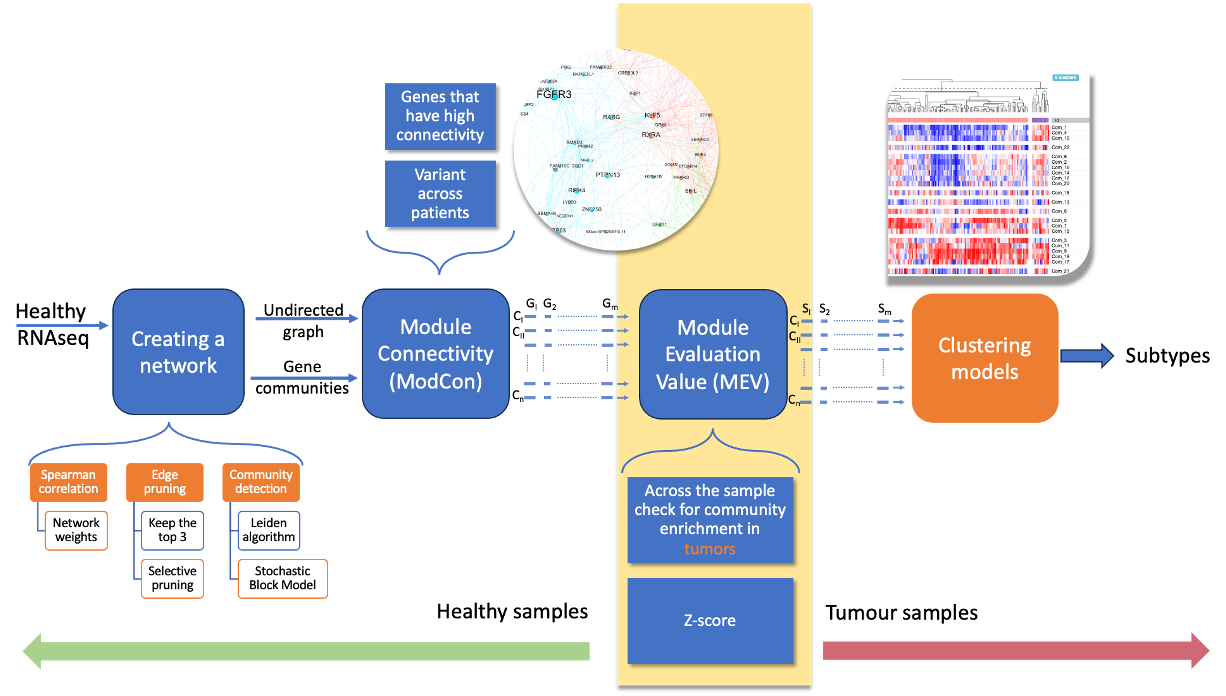
\includegraphics[width=0.75\textwidth,height=0.75\textheight,keepaspectratio]{Sections/Network_I/Resources/Methods/network_pipeline.png}
    \caption{Network pipene}
    \label{fig:N_I:network_pipeline}
\end{figure}



% \subsubsection{Building a network}

% \subsubsection{Analysing a network}

% \subsubsection{Finding communities}

% \subsubsection{Integrating data}

% \subsubsection{From gene communities back to samples subtypes}

% \subsubsection{Biological interpretation}